% Task 3 report: Research Results, Data Analysis and Scientific Visualisation.
% Numbers in the text come from generated_values.tex and generated_tables.tex (src/build_report.py).
% Build: latexmk -pdf -cd reports/latex/task3_report.tex
\documentclass[11pt,a4paper]{article}
\usepackage[utf8]{inputenc}
\usepackage[T1]{fontenc}
\usepackage{mathptmx}
\usepackage[scaled=0.92]{helvet}
\usepackage{courier}
\usepackage[margin=2.2cm]{geometry}
\usepackage{amsmath,amssymb}
\usepackage{booktabs}
\usepackage{graphicx}
\usepackage{caption}
\usepackage{subcaption}
\usepackage{xcolor}
\usepackage{microtype}
\usepackage[section]{placeins}
\usepackage[hidelinks]{hyperref}
\usepackage{url}
\captionsetup{font=small,labelfont=bf}
\graphicspath{{../figures/}}
% Generated by src/build_report.py -- do not edit by hand.
\newcommand{\vnMain}{285}
\newcommand{\vnA}{303}
\newcommand{\vnB}{327}
\newcommand{\vrhoMain}{0.283}
\newcommand{\vrhoMainLo}{0.177}
\newcommand{\vrhoMainHi}{0.384}
\newcommand{\vrhoA}{0.260}
\newcommand{\vrhoALo}{0.155}
\newcommand{\vrhoAHi}{0.363}
\newcommand{\vrhoB}{0.305}
\newcommand{\vrhoBLo}{0.205}
\newcommand{\vrhoBHi}{0.399}
\newcommand{\vpAsymMain}{1.2\times10^{-6}}
\newcommand{\vkwH}{26.4}
\newcommand{\vepsSq}{0.093}
\newcommand{\valphaC}{0.89}
\newcommand{\vrTwoBase}{0.004}
\newcommand{\vrTwoProp}{0.086}
\newcommand{\vdRTwo}{0.081}
\newcommand{\vFnested}{24.9}
\newcommand{\vpNested}{< 0.001}
\newcommand{\vbeta}{1.30}
\newcommand{\vbetaLo}{0.81}
\newcommand{\vbetaHi}{1.79}
\newcommand{\vbetaStd}{0.29}
\newcommand{\vbetaStdLo}{0.18}
\newcommand{\vbetaStdHi}{0.40}
\newcommand{\vcatDRTwo}{0.093}
\newcommand{\vshapiroP}{0.001}
\newcommand{\vbpP}{0.18}
\newcommand{\vnLog}{420}
\newcommand{\vnWarm}{60}
\newcommand{\vnBench}{360}
\newcommand{\vnInjected}{25}
\newcommand{\vnPaired}{155}
\newcommand{\vmaxDiff}{2.2e-16}
\newcommand{\vlatBase}{456.4}
\newcommand{\vlatVec}{47.2}
\newcommand{\vspeedTwoEightFive}{9.67}
\newcommand{\vspeedTwoEightFiveLo}{9.27}
\newcommand{\vspeedTwoEightFiveHi}{10.31}
\newcommand{\vspeedMin}{3.3}
\newcommand{\vspeedMax}{27.8}
\newcommand{\vspeedMinN}{2000}
\newcommand{\vspeedMaxN}{50}
\newcommand{\vcpu}{Intel(R) Xeon(R) Processor @ 2.80GHz}
\newcommand{\vncpu}{2}
\newcommand{\vpyBench}{3.12.3}

\newcommand{\repo}{\url{https://github.com/yernurkussain-source/TASK2_KUSSAIN_ZHAHYP}}

\title{Academic Generative AI Use and Unintentional Procrastination:\\ Task 3 Results, Data Analysis and Scientific Visualisation}
\author{Ernur Kussain \and Zhanassyl Zhakyp}
\date{2 November 2026}

\begin{document}
\maketitle

\begin{abstract}
We analysed a public survey of Indian bachelor's and master's students (Sharma et al., 2026) to test whether the frequency of academic generative-AI (GenAI) use is associated with unintentional procrastination. In the main sample ($n=\vnMain$), Spearman's $\hat\rho_s=\vrhoMain$ (95\% bootstrap CI \vrhoMainLo{} to \vrhoMainHi; $p<0.001$), so $H_0:\rho_s=0$ is rejected. Two sensitivity analyses on the raw file give $\hat\rho_s=\vrhoA$ and $\vrhoB$, and adding AI-use frequency to a covariates-only model raises $R^2$ from \vrTwoBase{} to \vrTwoProp{} (standardised $\beta=\vbetaStd$). A benchmark of the analysis pipeline, with warm-up filtering and error guardrails, shows that a vectorised bootstrap returns identical estimates and is \vspeedMin--\vspeedMax{} times faster than the Task~2 loop. The association is cross-sectional and may reflect stable traits rather than an effect of GenAI. No Kazakhstani study yet measures GenAI use together with procrastination, so we treat the result as a hypothesis for a local follow-up study, which we outline.
\end{abstract}

\section{Introduction}
Task~1 identified a gap: no study jointly examines purpose-specific GenAI use and validated procrastination measures among students in Kazakhstan, with attention to temporal order and confounders. Task~2 turned the association strand of that question into a testable hypothesis on open data:
\begin{equation}
H_0:\ \rho_s = 0 \qquad\text{vs.}\qquad H_1:\ \rho_s\neq0,\qquad \alpha=0.05\ \text{(two-sided)},
\label{eq:h0}
\end{equation}
where $\rho_s$ is the population Spearman correlation between academic GenAI-use frequency and the Unintentional Procrastination Scale (UPS) total. Task~3 collects and processes the data, formalises the domain model and reports the results. The repository is \repo; the release tagged \texttt{v1.0-task3} contains every file referred to here.

\section{Data and samples}
The source is Mendeley Data V1 (DOI 10.17632/88pv88j8jb.1, CC BY 4.0): a raw workbook with 355 responses and a cleaned workbook with 300. Both were downloaded and checked against the SHA-256 hashes stored in \path{configs/research.yaml}. All 300 UPS totals that we computed match the totals supplied by the authors. The main sample excludes 15 Higher Secondary respondents ($n=\vnMain$). Sensitivity~A applies our own rules to the raw file ($n=\vnA$); Sensitivity~B keeps respondents who use GenAI rarely or never as a reference level~0 ($n=\vnB$). Initials, academic-dishonesty items and domicile are never written to the derived files.

\section{Domain model}
\label{sec:domain}
We follow the ML/AI track: a formal definition of the target, the estimators, the loss function and the metrics. The full model, with a notation table and the code that implements each equation, is in \path{docs/domain_model.md}. For respondent $i$ with item answers $u_{ik}\in\{1,2,3,4\}$,
\begin{equation}
y_i = \sum_{k=1}^{6}\underbrace{u_{ik}}_{\text{UPS item}}\in\{6,\dots,24\},\qquad x_i\in\{1,2,3,4\}\ (\{0,\dots,4\}\text{ in Sensitivity B}).
\label{eq:ups}
\end{equation}

\paragraph{Primary metric.} With $R(\cdot)$ the average-rank transform,
\begin{equation}
\hat\rho_s=\frac{\sum_i\bigl(R(\mathbf x)_i-\bar R_x\bigr)\bigl(R(\mathbf y)_i-\bar R_y\bigr)}{\sqrt{\sum_i\bigl(R(\mathbf x)_i-\bar R_x\bigr)^2}\sqrt{\sum_i\bigl(R(\mathbf y)_i-\bar R_y\bigr)^2}}.
\label{eq:spearman}
\end{equation}
Uncertainty comes from $B=10\,000$ paired bootstrap resamples $I_b$:
\begin{equation}
\mathrm{CI}_{95\%}=\bigl[Q_{0.025}(\{\hat\rho^*_b\}),\,Q_{0.975}(\{\hat\rho^*_b\})\bigr],\qquad
v=\frac{|\mathcal B_{\text{valid}}|}{B}\ge0.95,
\label{eq:ci}
\end{equation}
and the permutation test uses
\begin{equation}
p_{\text{perm}}=\frac{1+\sum_{b=1}^{B}\mathbb 1\bigl[|\hat\rho_s(\mathbf x,\mathbf y_{\pi_b})|\ge|\hat\rho_s(\mathbf x,\mathbf y)|\bigr]}{B+1}.
\label{eq:perm}
\end{equation}

\paragraph{Loss function and models.} The supplementary regression compares a baseline $M_0$ with a proposed $M_1$,
\begin{equation}
M_0:\ y_i=\mathbf z_i^\top\gamma+\varepsilon_i,\qquad M_1:\ y_i=\mathbf z_i^\top\gamma+\beta x_i+\varepsilon_i,
\label{eq:models}
\end{equation}
fitted by minimising the squared-error loss
\begin{equation}
\mathcal L(\boldsymbol\theta)=\frac1n\sum_{i=1}^{n}\Bigl(\underbrace{y_i}_{\text{observed}}-\underbrace{\mathbf z_i^\top\gamma-\beta x_i}_{\text{predicted}}\Bigr)^2,\qquad
\hat{\boldsymbol\theta}=\arg\min_{\boldsymbol\theta}\mathcal L(\boldsymbol\theta).
\label{eq:loss}
\end{equation}
UPS is bounded in $[6,24]$, so squared error is not dominated by extreme values; the rank-based Eq.~\eqref{eq:spearman} stays the primary metric. Fit is compared with
\begin{equation}
\Delta R^2=R^2_1-R^2_0,\qquad F=\frac{\mathrm{SSR}_0-\mathrm{SSR}_1}{\mathrm{SSR}_1/(n-q-2)},
\label{eq:fit}
\end{equation}
and the interval for $\beta$ uses HC3 standard errors because the residuals are not normal.

\paragraph{Secondary metrics.} Kruskal--Wallis across $g$ use levels and Cliff's $\delta$ against the reference level $\ell_0$:
\begin{equation}
H=\frac{12}{n(n+1)}\sum_{\ell=1}^{g}n_\ell\bar R_\ell^{\,2}-3(n+1),\quad \varepsilon^2=\frac{H}{n-1};
\label{eq:kw}
\end{equation}
\begin{equation}
\delta_\ell=\frac{1}{|G_\ell||G_{\ell_0}|}\sum_{i\in G_\ell}\sum_{j\in G_{\ell_0}}\operatorname{sign}(y_i-y_j)\in[-1,1].
\label{eq:cliff}
\end{equation}

\paragraph{Pipeline metrics.} With $\mathcal R$ all timed runs and $\mathcal R_{\text{warm}}$ the warm-up runs,
\begin{equation}
\mathcal R_{\text{bench}}=\mathcal R\setminus\mathcal R_{\text{warm}},\qquad
\mathrm p q_{m,w}=Q_{q/100}\bigl(\{L_r: r\in\mathcal R_{\text{bench}},\ \text{status}_r=\text{ok},\ m_r=m,\ w_r=w\}\bigr),
\label{eq:bench}
\end{equation}
\begin{equation}
\mathcal S(w)=\frac{\mathrm p50_{\text{base},w}}{\mathrm p50_{\text{vec},w}},\qquad
e=\frac{|\mathcal R^{\text{error}}_{\text{bench}}|}{|\mathcal R_{\text{bench}}|}=0,\qquad
d=\frac{|\mathcal R^{\text{rejected}}|}{|\mathcal R^{\text{injected}}|}=1.
\label{eq:speedup}
\end{equation}

\begin{table}[!htbp]
\centering
\caption{Notation (abridged; the full table is in \texttt{docs/domain\_model.md}).}
\label{tab:notation}
\small
\begin{tabular}{@{}llll@{}}
\toprule
Symbol & Kind & Domain & Meaning\\
\midrule
$n$ & scalar & $\mathbb N$ & respondents in the analysed sample\\
$u_{ik}$ & scalar & $\{1,2,3,4\}$ & answer of respondent $i$ to UPS item $k$\\
$y_i$ & scalar & $\{6,\dots,24\}$ & UPS total (target)\\
$x_i$ & scalar & $\{0,\dots,4\}$ & academic GenAI-use frequency (exposure)\\
$\mathbf z_i$ & vector & $\mathbb R^{3}$ & covariates: age, gender, education\\
$\mathbf X_1$ & matrix & $\mathbb R^{n\times5}$ & design matrix of $M_1$ with intercept\\
$R(\cdot)$ & function & $\mathbb R^n\to\mathbb R^n$ & average-rank transform\\
$B$ & scalar & $10\,000$ & bootstrap and permutation resamples\\
$\mathcal L(\boldsymbol\theta)$ & function & $\mathbb R^{5}\to\mathbb R_{\ge0}$ & squared-error loss of the regression\\
$L_r$ & scalar & $\mathbb R_{>0}$, ms & latency of benchmark run $r$\\
$w$ & scalar & $\{50,\dots,2000\}$ & workload, records per run\\
\bottomrule
\end{tabular}
\end{table}

\paragraph{Architecture and threats.} Figure~\ref{fig:c4} places the six metric collection points (M1--M6) on a C4 container view of the pipeline, and \path{docs/domain_model.md} adds a STRIDE matrix for the data flow (for example, SHA-256 checks against spoofed source files and the exclusion of participant initials against information disclosure).

\begin{figure}[!htbp]
\centering
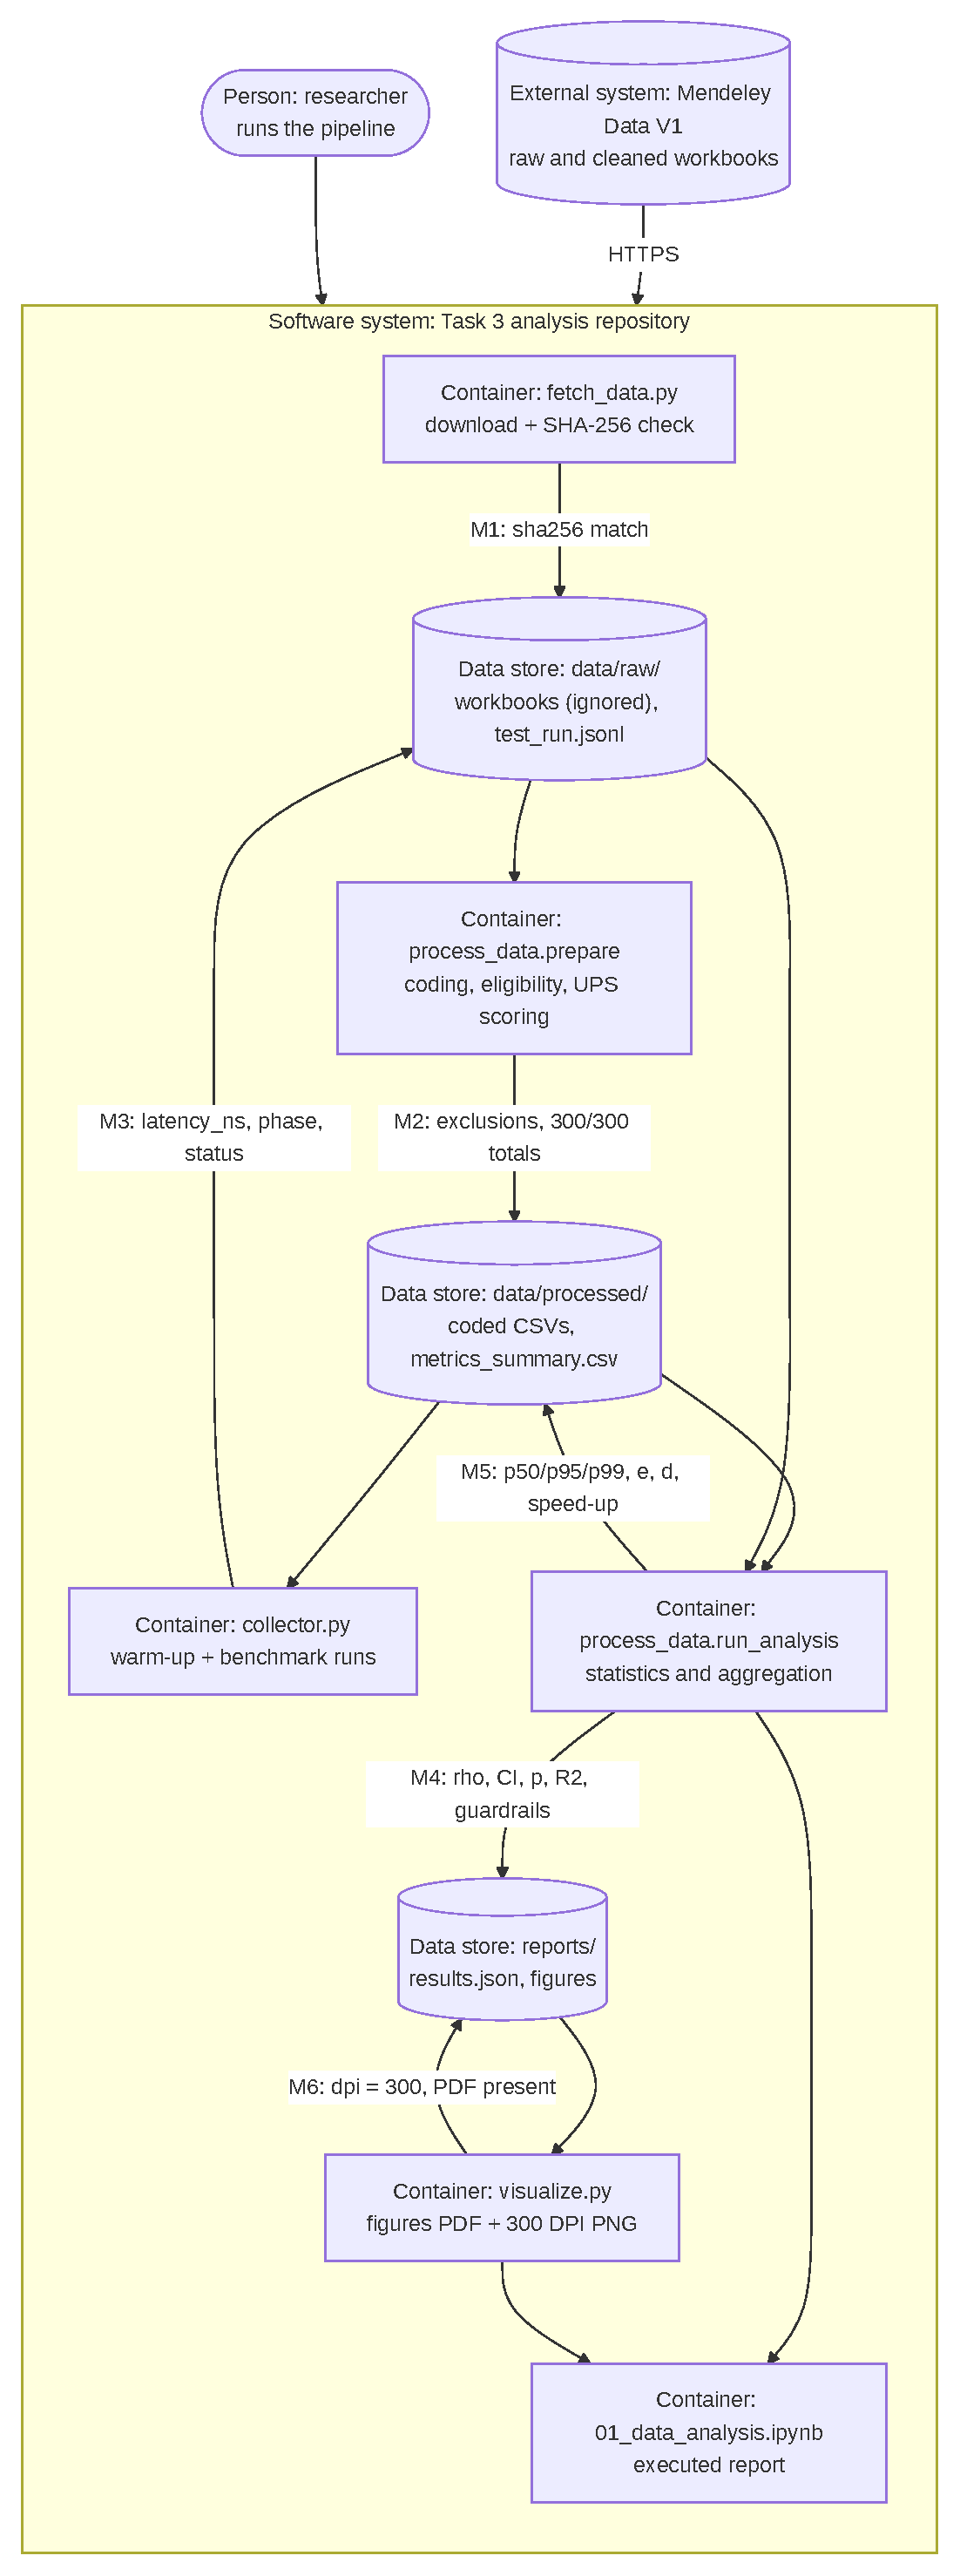
\includegraphics[height=0.72\textheight]{domain_c4_container.pdf}
\caption{C4 container view of the analysis repository. Arrows show data flow; labels M1--M6 are the points where metrics are recorded: hash checks (M1), exclusion counts and total audit (M2), per-run latency, phase and status (M3), survey statistics and guardrails (M4), latency percentiles, error and rejection rates and speed-up (M5), and figure checks (M6).}
\label{fig:c4}
\end{figure}

\section{Experimental results and discussion}
\label{sec:results}
\begin{table}[!htbp]
\centering
\caption{Primary association between academic GenAI-use frequency and UPS total (Eqs.~\ref{eq:spearman}--\ref{eq:perm}). Intervals are 95\% percentile bootstrap intervals ($B=10\,000$); $H$ and $\varepsilon^2$ come from the Kruskal--Wallis test across use levels (Eq.~\ref{eq:kw}). No column has a ``better'' direction, so no value is highlighted.}
\label{tab:association}
\footnotesize\setlength{\tabcolsep}{4pt}
\begin{tabular}{@{}lrlrrrr@{}}
\toprule
Analysis & $n$ & $\hat\rho_s$ [95\% CI] & $p_{\text{asym}}$ & $p_{\text{perm}}$ & $H$ & $\varepsilon^2$\\
\midrule

Main: supplied cleaned workbook & 285 & 0.283 [0.177, 0.384] & $1.2\times10^{-6}$ & $<0.001$ & 26.4 & 0.093\\

Sensitivity A: raw workbook, independent rules & 303 & 0.260 [0.155, 0.363] & $4.4\times10^{-6}$ & $<0.001$ & 23.7 & 0.078\\

Sensitivity B: raw workbook, five levels & 327 & 0.305 [0.205, 0.399] & $1.8\times10^{-8}$ & $<0.001$ & 34.0 & 0.104\\

\bottomrule
\end{tabular}
\end{table}

\begin{table}[!htbp]
\centering
\caption{UPS score by AI-use level and comparison with the lowest-use reference group. Values are Median (p25--p75) and Mean $\pm$ SD in UPS points. Median differences and Cliff's $\delta$ (Eq.~\ref{eq:cliff}) carry 95\% bootstrap intervals; $p$ values are Holm-adjusted Mann--Whitney tests. The largest $\delta$ in each sample is in bold.}
\label{tab:groups}
\footnotesize\setlength{\tabcolsep}{3.5pt}
\begin{tabular}{@{}lrllll r@{}}
\toprule
Use level & $n$ & Median (p25--p75) & Mean $\pm$ SD & $\Delta$ median [95\% CI] & $\delta$ [95\% CI] & $p_{\text{Holm}}$\\
\midrule

\multicolumn{7}{@{}l}{\emph{Main sample ($n=285$), reference = level 1}}\\

\quad 1: Few times a month & 81 & 12.0 (9--14) & 12.01 $\pm$ 4.29 & reference & reference & \\

\quad 2: Once a week & 39 & 14.0 (9--16) & 13.38 $\pm$ 4.23 & $+2.0$ [$+0.0$, $+5.0$] & 0.21 [-0.01, 0.42] & 0.067\\

\quad 3: Few times a week & 129 & 16.0 (12--19) & 15.24 $\pm$ 4.78 & $+4.0$ [$+2.0$, $+6.0$] & 0.39 [0.23, 0.53] & $<0.001$\\

\quad 4: Every day & 36 & 15.5 (12--17) & 14.94 $\pm$ 3.77 & $+3.5$ [$+2.0$, $+6.0$] & \textbf{0.41 [0.21, 0.60]} & $<0.001$\\

\multicolumn{7}{@{}l}{\emph{Sensitivity B ($n=327$), reference = level 0}}\\

\quad 0: Rarely/never & 24 & 10.5 (7--14) & 10.83 $\pm$ 4.11 & reference & reference & \\

\quad 1: Few times a month & 89 & 12.0 (9--15) & 12.29 $\pm$ 4.41 & $+1.5$ [$-2.0$, $+4.0$] & 0.19 [-0.08, 0.45] & 0.159\\

\quad 2: Once a week & 41 & 14.0 (9--16) & 13.44 $\pm$ 4.15 & $+3.5$ [$+0.0$, $+6.5$] & 0.36 [0.09, 0.62] & 0.032\\

\quad 3: Few times a week & 133 & 15.0 (12--19) & 15.20 $\pm$ 4.78 & $+4.5$ [$+2.0$, $+8.0$] & 0.51 [0.29, 0.69] & $<0.001$\\

\quad 4: Every day & 40 & 15.5 (12--17) & 14.90 $\pm$ 3.64 & $+5.0$ [$+2.0$, $+8.0$] & \textbf{0.54 [0.28, 0.76]} & $<0.001$\\

\bottomrule
\end{tabular}
\end{table}

\begin{table}[t]
\centering
\caption{Baseline model $M_0$ versus proposed model $M_1$ (Eqs.~\ref{eq:models}--\ref{eq:fit}), $n=285$. The better value of each criterion is in bold. Nested $F=24.9$, $p <0.001$; $\hat\beta=1.30$ UPS points per level (HC3 95\% CI 0.81 to 1.79).}
\label{tab:models}
\small
\begin{tabular}{@{}llrrrr@{}}
\toprule
Model & Predictors & $R^2$ & adj.\ $R^2$ & AIC & BIC\\
\midrule
$M_0$ baseline & age, gender, education & 0.004 & -0.006 & 1691.0 & 1705.6\\
$M_1$ proposed & $M_0$ + AI-use frequency & \textbf{0.086} & \textbf{0.072} & \textbf{1668.7} & \textbf{1687.0}\\
\bottomrule
\end{tabular}
\end{table}

\begin{table}[!htbp]
\centering
\caption{Pipeline latency per run (ms) after warm-up filtering, successful runs only (Eqs.~\ref{eq:bench}--\ref{eq:speedup}). Median (p25--p75) and tail percentiles for the Task~2 loop bootstrap (baseline) and the vectorised bootstrap (proposed), with the p50 speed-up $\mathcal{S}$ and its 95\% bootstrap interval. The lower (better) latency in each row is in bold.}
\label{tab:latency}
\footnotesize\setlength{\tabcolsep}{4pt}
\begin{tabular}{@{}r ll ll l@{}}
\toprule
& \multicolumn{2}{c}{Baseline (Task 2 loop)} & \multicolumn{2}{c}{Proposed (vectorised)} & \\
\cmidrule(lr){2-3}\cmidrule(lr){4-5}
$w$ & p50 (p25--p75) & p95 / p99 & p50 (p25--p75) & p95 / p99 & $\mathcal{S}$ [95\% CI]\\
\midrule

50 & 374.6 (360.4--393.1) & 430.7 / 435.2 & \textbf{13.5} (13.1--14.1) & \textbf{17.9 / 19.6} & 27.80 [27.02, 28.92]\\

100 & 398.5 (360.1--429.9) & 501.9 / 533.3 & \textbf{19.5} (18.9--21.0) & \textbf{29.3 / 29.9} & 20.44 [18.58, 21.76]\\

285 & 456.4 (445.9--483.3) & 524.8 / 551.5 & \textbf{47.2} (45.5--51.0) & \textbf{63.7 / 65.6} & 9.67 [9.27, 10.31]\\

500 & 496.2 (486.8--525.8) & 595.5 / 675.7 & \textbf{77.3} (74.7--78.5) & \textbf{85.6 / 87.6} & 6.41 [6.32, 6.67]\\

1000 & 648.8 (622.8--684.4) & 699.1 / 753.2 & \textbf{151.2} (144.7--155.8) & \textbf{167.8 / 171.3} & 4.29 [4.13, 4.53]\\

2000 & 905.3 (856.3--943.9) & 1065.0 / 1107.4 & \textbf{277.3} (252.6--293.5) & \textbf{324.7 / 348.1} & 3.26 [3.10, 3.41]\\

\bottomrule
\end{tabular}
\end{table}


\subsection{Primary association}
In the main sample, $\hat\rho_s=\vrhoMain$ (95\% CI \vrhoMainLo{} to \vrhoMainHi; asymptotic $p=\vpAsymMain$), and the permutation $p$ is at its floor of $1/(B+1)$ (Table~\ref{tab:association}). Sensitivity~A and B give \vrhoA{} and \vrhoB, so the authors' unexplained exclusions do not appear to drive the result. All bootstrap resamples were valid, and the UPS items were internally consistent (Cronbach's $\alpha=\valphaC$). Figure~\ref{fig:dist} shows the distributions.

\begin{figure}[!htbp]
\centering
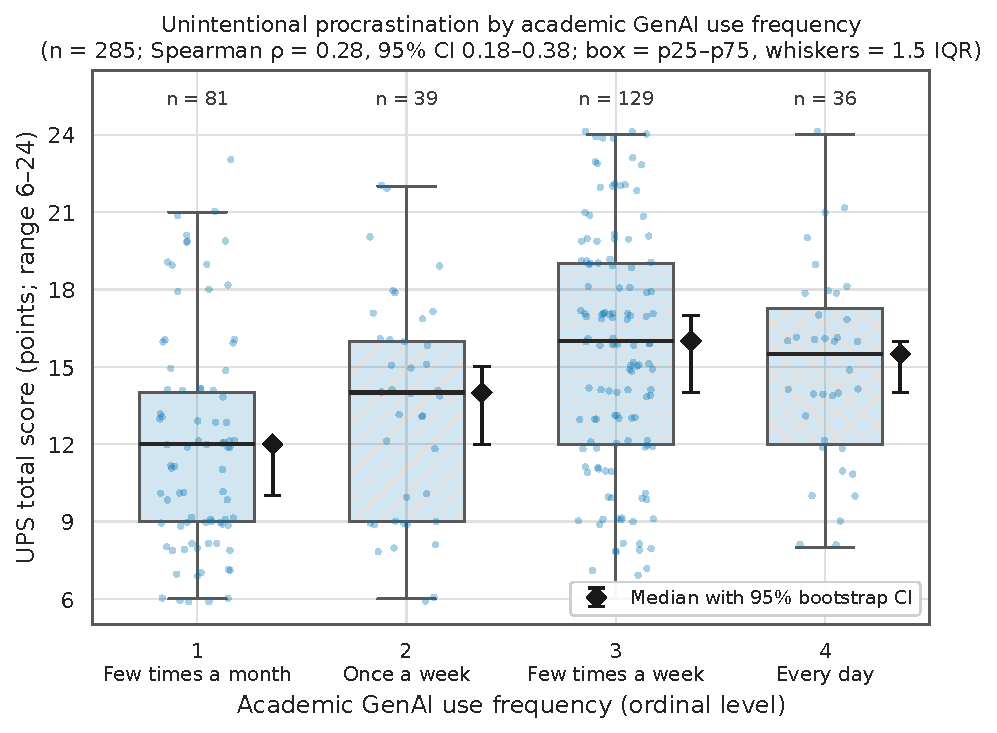
\includegraphics[width=0.82\textwidth]{fig2_distribution_boxplot.pdf}
\caption{UPS totals (points, range 6--24) by academic GenAI-use level, main sample ($n=\vnMain$). Boxes span p25--p75 and whiskers 1.5\,IQR; points are jittered respondents; diamonds are medians with 95\% bootstrap intervals (10\,000 resamples). Scores rise from monthly to a-few-times-a-week use and level off for daily users.}
\label{fig:dist}
\end{figure}

\subsection{Reference-group comparison}
Respondents who use GenAI a few times a week or every day score 3--4 points higher than the monthly reference group and 4--5 points higher than the rarely/never group (Table~\ref{tab:groups}, Figure~\ref{fig:panels}a). Weekly users do not differ clearly from monthly users. Cliff's $\delta$ for the two highest levels (about 0.4--0.5) is medium to large.

\subsection{Baseline versus proposed model}
Age, gender and education explain almost none of the variance ($R^2=\vrTwoBase$). Adding AI-use frequency raises $R^2$ to \vrTwoProp{} ($\Delta R^2=\vdRTwo$, nested $F=\vFnested$; Table~\ref{tab:models}). The coefficient is $\hat\beta=\vbeta$ UPS points per level (HC3 95\% CI \vbetaLo{} to \vbetaHi), or $\beta_{\text{std}}=\vbetaStd$ (\vbetaStdLo{} to \vbetaStdHi), close to the $\beta=0.309$ reported by Abbas et al.\ (2024) for ChatGPT use and a general procrastination measure. A categorical coding of frequency gives a similar gain ($\Delta R^2=\vcatDRTwo$). Residuals are not normal (Shapiro--Wilk $p=\vshapiroP$); the Breusch--Pagan test does not indicate heteroscedasticity ($p=\vbpP$).

\subsection{Pipeline benchmark}
The log holds \vnLog{} timed runs; \vnWarm{} warm-up runs were discarded and \vnBench{} benchmark runs analysed (\vcpu, \vncpu{} logical CPUs, Python \vpyBench). On \vnPaired{} paired runs with identical inputs, the two implementations returned the same estimates (largest absolute difference \vmaxDiff). The vectorised bootstrap was faster at every workload, from \vspeedMin$\times$ at \vspeedMinN{} records to \vspeedMax$\times$ at \vspeedMaxN{} records; at 285 records the median run fell from \vlatBase{} to \vlatVec{} ms ($\mathcal S=\vspeedTwoEightFive$, 95\% CI \vspeedTwoEightFiveLo--\vspeedTwoEightFiveHi; Table~\ref{tab:latency}, Figures~\ref{fig:warmup} and~\ref{fig:panels}c--d). No unexpected error occurred, and all \vnInjected{} injected invalid batches were rejected, so $e=0$ and $d=1$ in Eq.~\eqref{eq:speedup}.

\begin{figure}[!htbp]
\centering
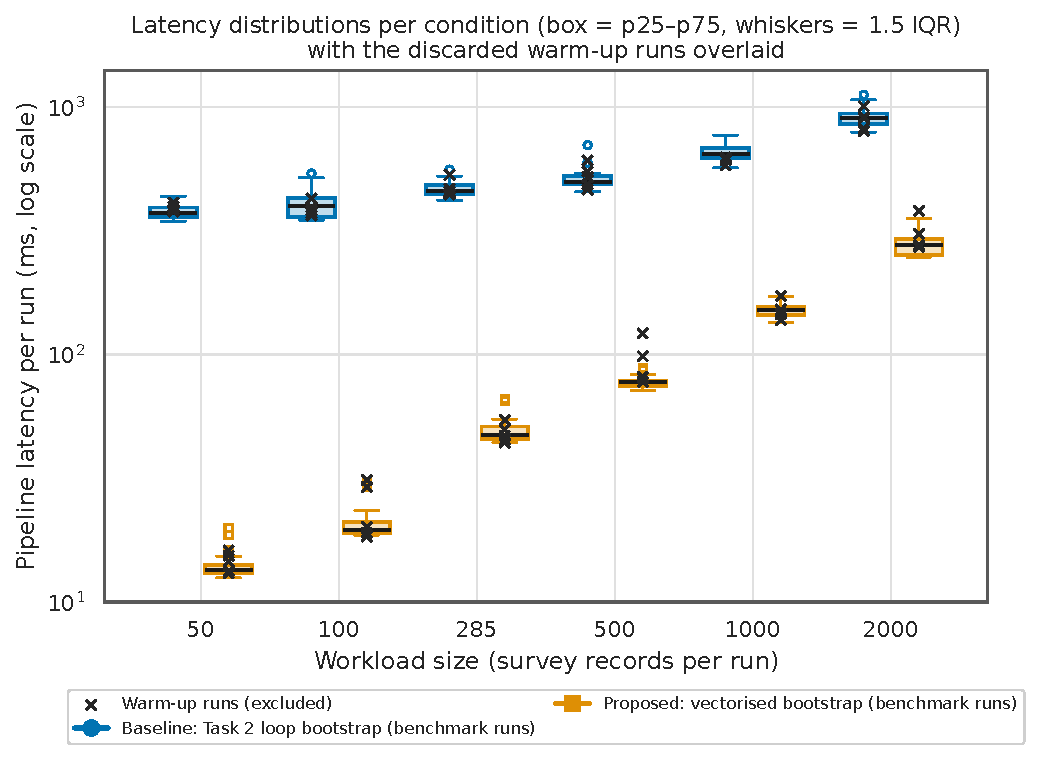
\includegraphics[width=0.78\textwidth]{fig5_latency_distribution.pdf}
\caption{Latency per run (ms, log scale) of the benchmark runs for each workload and implementation: boxes span p25--p75, whiskers reach 1.5\,IQR, and outliers are flagged but kept. Black crosses are the warm-up runs, which are logged but excluded from every statistic. Cold runs were at most about 1.6 times the benchmark median, so the warm-up effect is small in this pipeline.}
\label{fig:warmup}
\end{figure}

\begin{figure}[!htbp]
\centering
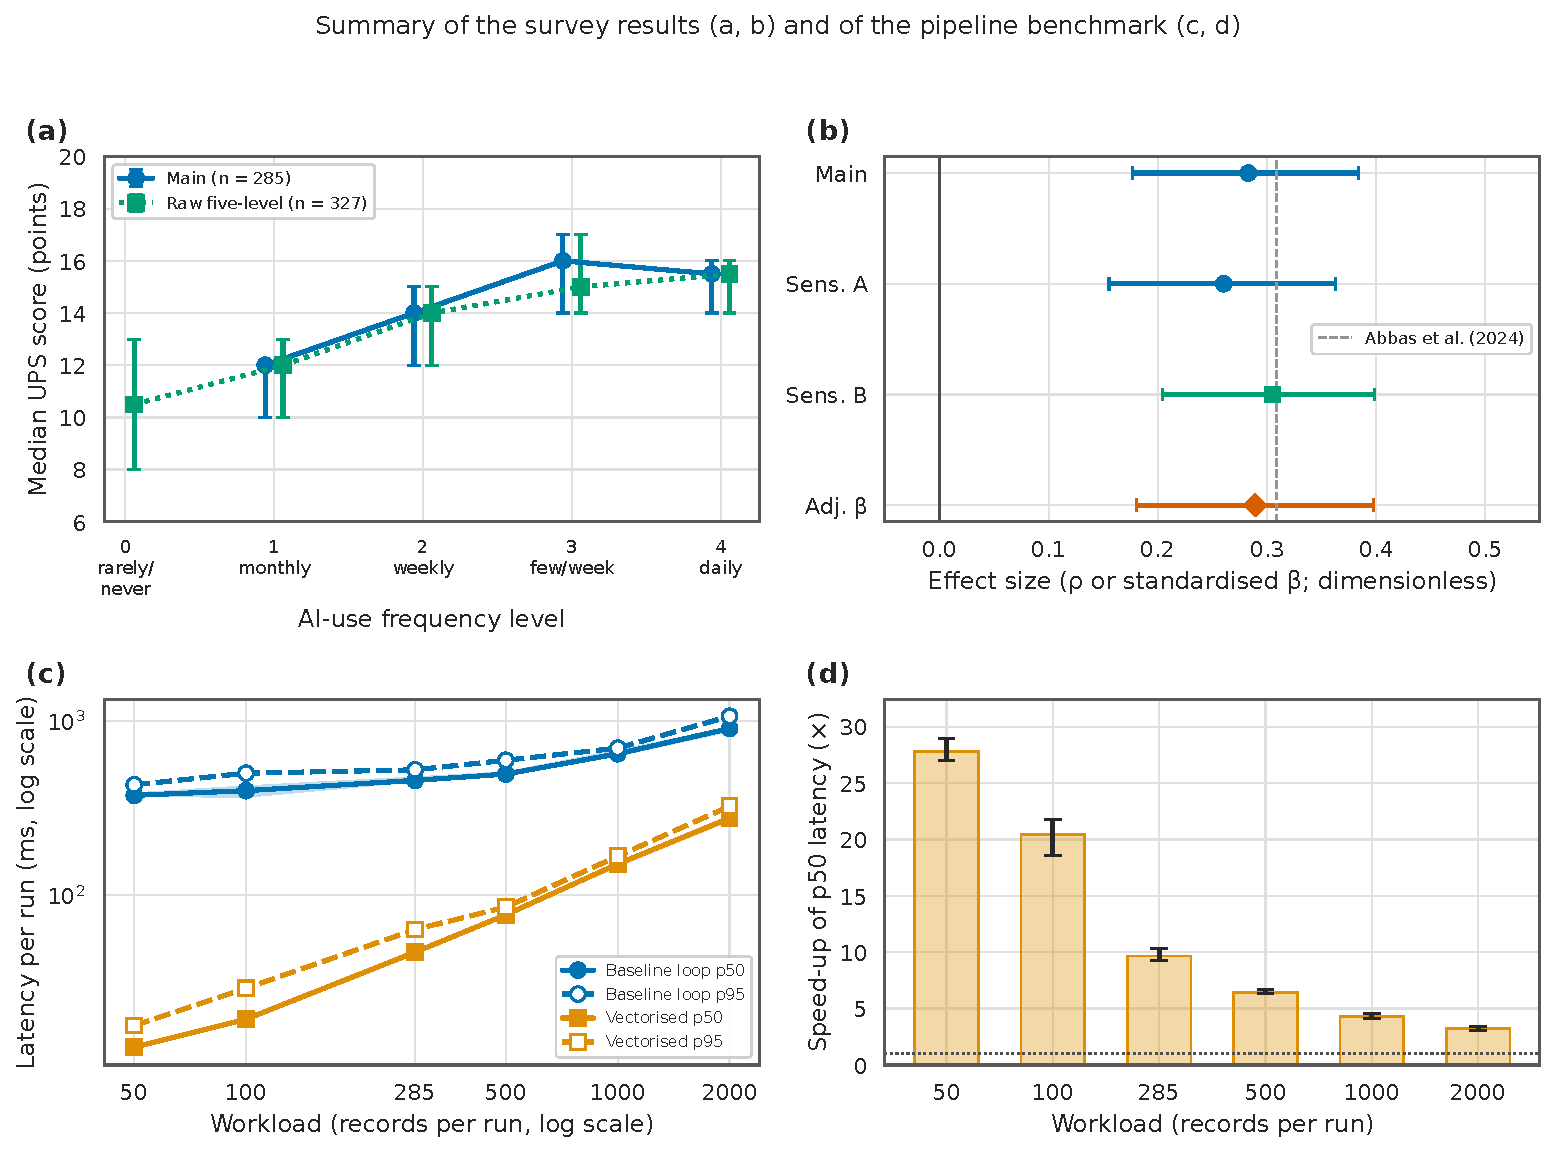
\includegraphics[width=\textwidth]{fig6_summary_panels.pdf}
\caption{Summary of the survey results and the pipeline benchmark. (a) Median UPS score (points) per AI-use level in the main and five-level samples; error bars are 95\% bootstrap intervals. (b) Effect sizes with 95\% intervals: Spearman $\rho$ for the main and sensitivity analyses and the standardised $\beta$ of $M_1$; the solid line is the null baseline and the dashed line Abbas et al.\ (2024). (c) p50 (solid) and p95 (dashed) latency (ms, log scale) against workload; shaded bands are 95\% bootstrap intervals of p50; warm-up runs are excluded. (d) p50 speed-up of the vectorised implementation with 95\% bootstrap intervals; the dotted line marks no speed-up.}
\label{fig:panels}
\end{figure}

\subsection{Discussion}
The size of the association is close to the 75th percentile of correlations in individual-differences research (Gignac \& Szodorai, 2016) and within the range of recent studies of GenAI use or dependence and procrastination, about 0.23--0.43 (Abbas et al., 2024; Galindo-Dom\'inguez et al., 2026; Liu \& Liu, 2026). It still explains only about 8\% of the variance. The design cannot show direction. In the one baseline-adjusted three-wave panel we found, GenAI-use frequency did not predict later procrastination ($\beta=0.007$; Zhao et al., 2026). The UPS correlates 0.78 with general procrastination and about 0.5 with depression and anxiety (Fernie et al., 2017), so stable traits and distress, which the source data do not measure, may account for part of the association.

\section{Relevance to Kazakhstan}
\label{sec:kz}
\paragraph{What is known.} We found no Kazakhstani study that measures GenAI use together with procrastination, time management or self-regulation. GenAI use is widespread: in a 2024 survey of 840 students at three universities, 65\% used AI tools for study at least weekly, mainly for essays, problem solving and ideas (Zhunusbekova \& Askarkyzy, 2024; abstract-level evidence). In 77 teacher-education students, 76 used AI, mostly to summarise checked readings and to draft outlines (Yrymbayeva et al., 2026). At one university, AI-use frequency was not related to GPA ($n=110$; Aubakirov, 2026, conference listing), and in Uzbekistan self-regulation, not AI-use intensity, predicted students' AI-related competence (Zaripova et al., 2026). The only Kazakhstani procrastination study whose content we could check used a modified Tuckman scale with 72 students (Journal of Educational Sciences, 2021). No Kazakh or Russian version of the UPS exists.

\paragraph{Policy context.} The national AI Concept 2024--2029 and Law No.~230-VIII ``On Artificial Intelligence'' (in force from 18 January 2026) do not regulate students' coursework. The Ministry of Science and Higher Education does not support a ban; it asks students to cite AI use and leaves integrity rules to universities, which differ widely. At the same time AI courses are compulsory, and the AI-Sana programme reported more than 600\,000 students and 671\,557 certificates in its first stage (press and ministry statements; dated sources are listed in \path{reports/kazakhstan_context.md}).

\paragraph{Implications for transfer.} Four differences make a direct transfer of $\hat\rho_s=\vrhoMain$ unlikely. (1) With near-universal use, a four-level frequency item will cluster at the top, and the correlation will weaken through range restriction. (2) Where AI use is part of the curriculum, frequency partly reflects course demands rather than personal habit, so the type of use and dependence become more informative. (3) Without a validated Kazakh or Russian UPS, scores cannot be compared across language groups, and a trilingual Kazakhstani survey found that answers differ by language (Issakhanova et al., 2026). (4) Confounders such as distress and workload must be measured, and the roughly 9\,300 Indian students in Kazakhstan should be analysed as a separate stratum.

\paragraph{Proposed follow-up study.} Translate and validate the UPS in Kazakh and Russian (back-translation, cognitive interviews, confirmatory factor analysis, measurement invariance). Measure the four-level frequency item, the eight-item ChatGPT scale of Abbas et al.\ (2024), a dependence scale and the type of use, together with depression, anxiety, workload and self-regulation. Collect three waves at universities with different AI policies. Detecting $\rho_s=0.18$ (the lower bound of our interval) with 80\% power at $\alpha=0.05$ needs about 240 complete cases (Fisher $z$); with the retention of 65.7\% seen by Zhao et al.\ (2026), about 365 students are needed at the first wave.

\section{Limitations}
The data are cross-sectional self-reports from a convenience sample recruited online in India, collected for a study of academic dishonesty; our analysis is secondary. The UPS measures unintentional procrastination in general rather than academic procrastination. The frequency item is ordinal, so the linear term in $M_1$ is an approximation. The benchmark timings come from one machine and are engineering diagnostics, not research outcomes.

\section{Reproducibility}
All parameters, hashes and the seed (20261007) are in \path{configs/research.yaml}. From a fresh checkout:
{\footnotesize
\begin{verbatim}
python -m pip install -r requirements.txt
python -m unittest discover -s tests -v
python src/run_pipeline.py
jupyter nbconvert --to notebook --execute --inplace notebooks/01_data_analysis.ipynb
python src/build_report.py && latexmk -pdf -cd reports/latex/task3_report.tex
\end{verbatim}
}
Figures are written as vector PDF and 300~DPI PNG to \path{reports/figures/}; the executed notebook is \path{notebooks/01_data_analysis.ipynb}.

\begin{thebibliography}{99}\small
\bibitem{abbas} Abbas, M., Jam, F.\,A., \& Khan, T.\,I. (2024). Is it harmful or helpful? Examining the causes and consequences of generative AI usage among university students. \emph{International Journal of Educational Technology in Higher Education}, 21, 10. \url{https://doi.org/10.1186/s41239-024-00444-7}
\bibitem{aubakirov} Aubakirov, A. (2026). Does generative AI improve academic performance? Evidence from higher education in Kazakhstan. NeurIPS 2026 virtual site listing. \url{https://neurips.cc/virtual/2026/175377}
\bibitem{fernie} Fernie, B.\,A., Bharucha, Z., Nik\v{c}evi\'c, A.\,V., \& Spada, M.\,M. (2017). The Unintentional Procrastination Scale. \emph{Journal of Rational-Emotive \& Cognitive-Behavior Therapy}, 35, 136--149. \url{https://doi.org/10.1007/s10942-016-0247-x}
\bibitem{galindo} Galindo-Dom\'inguez, H., Sainz-de-la-Maza, M., Campo, L., \& Losada-Iglesias, D. (2026). The influence of learning motivation and procrastination on ChatGPT dependence. \emph{RIED-Revista Iberoamericana de Educaci\'on a Distancia}, 29(1), 217--240. \url{https://doi.org/10.5944/ried.45497}
\bibitem{gignac} Gignac, G.\,E., \& Szodorai, E.\,T. (2016). Effect size guidelines for individual differences researchers. \emph{Personality and Individual Differences}, 102, 74--78. \url{https://doi.org/10.1016/j.paid.2016.06.069}
\bibitem{issakhanova} Issakhanova, A., Abdullina, G., \& Belessova, N. (2026). Structural barriers to university counselling and ChatGPT as a preferred help-seeking alternative: A convergent mixed-methods study among Generation Z students in Kazakhstan. \emph{Frontiers in Education}, 11, 1838533. \url{https://doi.org/10.3389/feduc.2026.1838533}
\bibitem{jes} Academic procrastination of masters of the university in the conditions of the COVID-19 pandemic. (2021). \emph{Journal of Educational Sciences (Bulletin of KazNU)}, 66(1), 35--40. \url{https://doi.org/10.26577/JES.2021.v66.i1.04}
\bibitem{liu} Liu, Y., \& Liu, Y. (2026). Association between perceived usefulness of generative AI for learning and generative AI dependency among university students in Changde, China. \emph{Frontiers in Psychology}, 17, 1859317. \url{https://doi.org/10.3389/fpsyg.2026.1859317}
\bibitem{sharma} Sharma, P., Nandy, D., Ramchandani, G., James, A., Batra, M., \& Dhanda, R. (2026). \emph{Datasheets for Role of Generative Artificial Intelligence Usage on Academic Dishonesty Among Indian Undergraduate and Postgraduate Students} (Version 1) [Data set]. Mendeley Data. \url{https://doi.org/10.17632/88pv88j8jb.1}
\bibitem{yrym} Yrymbayeva, N., Yermekova, M., Tezekova, O., Issatayeva, B., Zhubandykova, A., \& Tuxanbayev, A. (2026). Information competence and critical thinking in digital environments: Evidence from university students in Kazakhstan. \emph{Frontiers in Education}, 11, 1809360. \url{https://doi.org/10.3389/feduc.2026.1809360}
\bibitem{zaripova} Zaripova, D., Zohirov, K., Rasulova, N., Khayitov, U., Saidova, D., Temirov, Z., \& Nasimov, R. (2026). Generative AI use, self-regulation, and Neuro-AI pedagogical competence in higher education: A comparative study of undergraduate and graduate students in Uzbekistan. \emph{Frontiers in Education}, 11, 1846709. \url{https://doi.org/10.3389/feduc.2026.1846709}
\bibitem{zhao} Zhao, Y., Chen, J., Dai, W., \& Gu, Y. (2026). Learning-centred use of generative AI and later academic functioning: A baseline-adjusted three-wave panel study. \emph{Frontiers in Psychology}, 17, 1878514. \url{https://doi.org/10.3389/fpsyg.2026.1878514}
\bibitem{zhun} Zhunusbekova, A., \& Askarkyzy, S. (2024). Students' perceptions of artificial intelligence use in higher education and its impact on academic integrity. \emph{Pedagogy and Psychology}, 61(4), 145--155. \url{https://doi.org/10.51889/2960-1649.2024.61.4.008}
\end{thebibliography}
\end{document}
